% !TEX program = pdflatex
\documentclass[aspectratio=169,10pt]{beamer}

\usetheme[progressbar=frametitle]{metropolis}
\setbeamertemplate{frame numbering}[fraction]
\metroset{block=fill}

\usepackage[utf8]{inputenc}
\usepackage[T1]{fontenc}
\usepackage[slovene]{babel}
\usepackage{microtype}
\usepackage{amsmath, amssymb, amsthm}
\usepackage{booktabs}
\usepackage{tikz}
\usetikzlibrary{positioning,fit,backgrounds,arrows.meta}
\usepackage{xcolor}

% Convenience macros that match the paper.
\newcommand{\rfmm}[3]{\omega(#1,#2,#3)}
\newcommand{\bigO}{O}

% Title-page data.
\title{Štetje 4-ciklov v polno dinamičnih grafih}
\subtitle{Z vidika cikličnih stikov}
\author{Govorec 1 \and Govorec 2 \and Govorec 3 \and Govorec 4}
\institute{Seminar iz algoritmov -- poskusna predstavitev za PODS 2025}
\date{}

\begin{document}

% ---------------------------------------------------------------
\begin{frame}[plain]
  \titlepage
\end{frame}

% =========================================================================
% Govorec 1 -- Problem (3:30)
% =========================================================================

% ---------------------------------------------------------------
\begin{frame}{Motivacijski primer: ciklični vzorci v grafu transakcij}
  \begin{columns}[T,onlytextwidth]
    \begin{column}{0.42\textwidth}
      \centering
      \vspace{0.3em}
      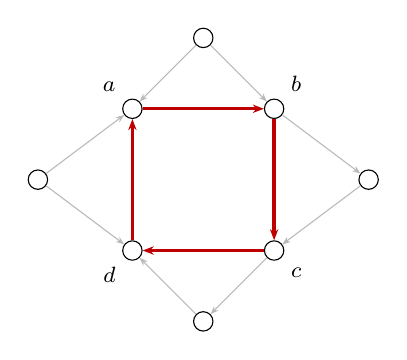
\begin{tikzpicture}[
          every node/.style={font=\footnotesize},
          vert/.style={circle,draw,inner sep=1.5pt,minimum size=7pt,fill=white},
          cedge/.style={red!75!black,very thick,-{Stealth[length=4pt]}},
          eedge/.style={gray!55,thin,-{Stealth[length=3pt]}},
        ]
        \node[vert,label=above left:$a$]  (a) at (0, 1.8) {};
        \node[vert,label=above right:$b$] (b) at (1.8, 1.8) {};
        \node[vert,label=below right:$c$] (c) at (1.8, 0.0) {};
        \node[vert,label=below left:$d$]  (d) at (0, 0.0) {};
        \node[vert] (e) at (-1.2, 0.9) {};
        \node[vert] (f) at (3.0, 0.9) {};
        \node[vert] (g) at (0.9, 2.7) {};
        \node[vert] (h) at (0.9, -0.9) {};
        \draw[eedge] (e) -- (a);
        \draw[eedge] (e) -- (d);
        \draw[eedge] (b) -- (f);
        \draw[eedge] (f) -- (c);
        \draw[eedge] (g) -- (a);
        \draw[eedge] (g) -- (b);
        \draw[eedge] (h) -- (d);
        \draw[eedge] (c) -- (h);
        \draw[cedge] (a) -- (b);
        \draw[cedge] (b) -- (c);
        \draw[cedge] (c) -- (d);
        \draw[cedge] (d) -- (a);
      \end{tikzpicture}

      \vspace{0.4em}
      {\scriptsize\emph{računi (vozlišča), transakcije (puščice)}}
    \end{column}
    \begin{column}{0.58\textwidth}
      Z računa $a$ gre nakazilo na račun $b$, z $b$ na $c$, s $c$ na $d$ in z $d$ nazaj na $a$ -- to je \alert{4-cikel v grafu transakcij} in značilen vzorec pri odkrivanju goljufij.

      \medskip
      Formalno gre za \alert{ciklično konjunktivno poizvedbo}: štiri relacije, sklenjene v zanko. Število rezultatov poizvedbe je natanko število 4-ciklov v grafu.

      \medskip
      Enaka struktura se pojavlja v številnih primerih -- cikli citatov, skupine, ki si vzajemno sledijo na družbenih omrežjih, priporočilne zanke.

      \medskip
      \alert{Pri tem se graf neprestano spreminja.}
    \end{column}
  \end{columns}
\end{frame}

% ---------------------------------------------------------------
\begin{frame}{Polno dinamično okolje}
  Vsaka nova transakcija doda eno povezavo; prav tako so dovoljena brisanja. Po \emph{vsaki} posodobitvi mora sistem sporočiti natančno število 4-ciklov.

  \vspace{0.6em}
  Ponovno izračunavanje od začetka je za velike grafe predrago. Potrebujemo hitro posodabljanje pri vsaki spremembi.

  \vspace{0.6em}
  \begin{block}{V najslabšem primeru, ne amortizirano}
    Strošek, ki ga merimo, je čas \emph{najpočasnejše} posodobitve -- ne pa povprečje čez celotno zaporedje posodobitev.

    \medskip
    Sistemi podatkovnih baz so občutljivi na repne zakasnitve: že ena sama posodobitev, dolga sekundo, je za produkcijo težava, čeprav je povprečje hitro.
  \end{block}

  \vspace{0.6em}
  Cilj je torej ambiciozen: biti hitrejši od ponovnega izračuna od začetka, in to z zagotovilom o najslabšem primeru za vsako posamezno posodobitev.
\end{frame}

% =========================================================================
% Govorec 2 -- Stanje stroke in presenečenje hitrega množenja matrik (3:30)
% =========================================================================

% ---------------------------------------------------------------
\begin{frame}{Pokrajina: trije majhni vzorci}
  Doslej najboljši strošek vzdrževanja na posodobitev za posamezen vzorec:

  \vspace{0.6em}
  \centering
  \begin{tabular}{lcc}
    \toprule
    Vzorec & Oblika & Najboljši strošek na posodobitev \\
    \midrule
    Trikotnik (3-cikel) &
      \raisebox{-0.4\height}{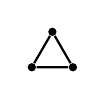
\begin{tikzpicture}[scale=0.30]
        \node[circle,fill=black,inner sep=0pt,minimum size=3pt] (a) at (0,1) {};
        \node[circle,fill=black,inner sep=0pt,minimum size=3pt] (b) at (-0.87,-0.5) {};
        \node[circle,fill=black,inner sep=0pt,minimum size=3pt] (c) at (0.87,-0.5) {};
        \draw[thick] (a)--(b)--(c)--(a);
      \end{tikzpicture}}
      & $\sqrt{m}$ \\
    4-klika &
      \raisebox{-0.4\height}{
\begin{tikzpicture}[scale=0.30]
        \node[circle,fill=black,inner sep=0pt,minimum size=3pt] (a) at (0,1) {};
        \node[circle,fill=black,inner sep=0pt,minimum size=3pt] (b) at (1,0) {};
        \node[circle,fill=black,inner sep=0pt,minimum size=3pt] (c) at (0,-1) {};
        \node[circle,fill=black,inner sep=0pt,minimum size=3pt] (d) at (-1,0) {};
        \draw[thick] (a)--(b)--(c)--(d)--(a);
        \draw[thick] (a)--(c); \draw[thick] (b)--(d);
      \end{tikzpicture}}
      & $m$ \\
    \alert{4-cikel} &
      \raisebox{-0.4\height}{
\begin{tikzpicture}[scale=0.30]
        \node[circle,fill=red!70!black,inner sep=0pt,minimum size=3pt] (a) at (0,1) {};
        \node[circle,fill=red!70!black,inner sep=0pt,minimum size=3pt] (b) at (1,0) {};
        \node[circle,fill=red!70!black,inner sep=0pt,minimum size=3pt] (c) at (0,-1) {};
        \node[circle,fill=red!70!black,inner sep=0pt,minimum size=3pt] (d) at (-1,0) {};
        \draw[thick,red!70!black] (a)--(b)--(c)--(d)--(a);
      \end{tikzpicture}}
      & \alert{$m^{2/3}$} \\
    \bottomrule
  \end{tabular}

  \vspace{1.0em}
  \raggedright
  \begin{itemize}
    \item Trikotniki in 4-klike imajo jasne, naravne eksponente.
    \item \alert{4-cikli imajo nenavaden eksponent $2/3$} -- niti kvadratni koren niti linearno.
    \item Meja $2/3$ je veljala za najboljši znani rezultat \alert{več kot desetletje}.
  \end{itemize}
\end{frame}

% ---------------------------------------------------------------
\begin{frame}{Od kod izvira meja $m^{2/3}$?}
  \begin{columns}[T,onlytextwidth]
    \begin{column}{0.62\textwidth}
      Vsak algoritem v tem prostoru izkorišča isto opazko: stopnje vozlišč so zelo različne.

      \vspace{0.6em}
      \begin{itemize}
        \item Malo \alert{vozlišč visoke stopnje} (npr.\ banke, veliki trgovci); obdelava vsakega je draga.
        \item Veliko \alert{vozlišč nizke stopnje}; vsako zase je poceni.
      \end{itemize}

      \vspace{0.6em}
      Če 4-cikle štejemo ločeno za oba razreda in prag izberemo tako, da se stroška uravnotežita, dobimo natanko $m^{2/3}$.

      \vspace{0.6em}
      To je \alert{naravna zgornja meja} za vsak kombinatorični algoritem, ki povezave obdeluje posamično.
    \end{column}
    \begin{column}{0.36\textwidth}
      \centering
      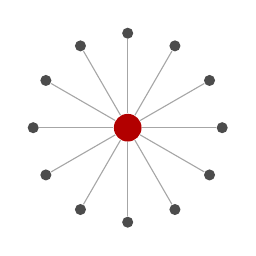
\begin{tikzpicture}[
          every node/.style={font=\scriptsize},
          hub/.style={circle,fill=red!70!black,inner sep=0pt,minimum size=10pt},
          small/.style={circle,fill=black!70,inner sep=0pt,minimum size=4pt},
        ]
        \node[hub] (h) at (0,0) {};
        \foreach \a in {0,30,60,90,120,150,180,210,240,270,300,330} {
          \node[small] (s\a) at ({1.2*cos(\a)}, {1.2*sin(\a)}) {};
          \draw[gray!70,thin] (h) -- (s\a);
        }
      \end{tikzpicture}

      {\scriptsize visoka stopnja: eno vozlišče, veliko povezav}

      \vspace{0.8em}
      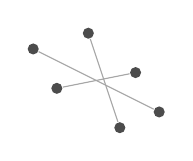
\begin{tikzpicture}[
          every node/.style={font=\scriptsize},
          small/.style={circle,fill=black!70,inner sep=0pt,minimum size=4pt},
        ]
        \node[small] (na) at (0,0)      {};
        \node[small] (nb) at (1,0.2)    {};
        \node[small] (nc) at (0.4,0.7)  {};
        \node[small] (nd) at (0.8,-0.5) {};
        \node[small] (ne) at (-0.3,0.5) {};
        \node[small] (nf) at (1.3,-0.3) {};
        \draw[gray!70,thin] (na) -- (nb);
        \draw[gray!70,thin] (nc) -- (nd);
        \draw[gray!70,thin] (ne) -- (nf);
      \end{tikzpicture}

      {\scriptsize nizka stopnja: veliko vozlišč, malo povezav}
    \end{column}
  \end{columns}
\end{frame}

% ---------------------------------------------------------------
\begin{frame}{Rezultat Assadija in Shaha (2025)}
  Assadi in Shah (PODS 2025) sta končno presegla to mejo: dosegla sta čas posodobitve $m^{2/3-\varepsilon}$ v najslabšem primeru, za neko konstanto $\varepsilon > 0$.

  \vspace{0.4em}
  Nepričakovana sestavina: \alert{hitro množenje matrik}.

  \vspace{0.6em}
  Zakaj je to presenetljivo?
  \begin{itemize}
    \item Hitro množenje matrik je \alert{množična} operacija -- učinkovita je le, če imamo na voljo dve veliki matriki in ju pomnožimo naenkrat.
    \item Naš problem je nasproten, \alert{tokovni} -- povezave prihajajo posamično, ena za drugo.
    \item V stroki je veljalo, da sta pristopa nezdružljiva.
  \end{itemize}

  \vspace{0.4em}
  \begin{block}{Uskladitev: faze}
    Tok posodobitev razdelimo v faze. Med vsako fazo algoritem na poizvedbe odgovarja s pomočjo produkta matrik, izračunanega v prejšnji fazi, medtem ko se naslednji produkt sproti računa v ozadju -- strošek je porazdeljen čez celotno fazo. Ob koncu faze se produkta zamenjata.
  \end{block}
\end{frame}

% =========================================================================
% Govorec 3 -- Naš prispevek (3:30)
% =========================================================================

% ---------------------------------------------------------------
\begin{frame}{Zakaj množenje matrik?}
  \begin{columns}[T,onlytextwidth]
    \begin{column}{0.42\textwidth}
      \centering
      \vspace{0.8em}
      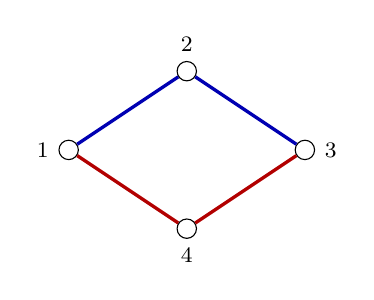
\begin{tikzpicture}[
          every node/.style={font=\footnotesize},
          vert/.style={circle,draw,inner sep=1.5pt,minimum size=7pt,fill=white},
          tedge/.style={blue!70!black,very thick},
          bedge/.style={red!70!black,very thick},
        ]
        \node[vert,label=left:$1$]   (a) at (0, 0)    {};
        \node[vert,label=above:$2$]  (b) at (1.5, 1)  {};
        \node[vert,label=right:$3$]  (c) at (3, 0)    {};
        \node[vert,label=below:$4$]  (d) at (1.5,-1)  {};
        \draw[tedge] (a) -- (b);
        \draw[tedge] (b) -- (c);
        \draw[bedge] (a) -- (d);
        \draw[bedge] (d) -- (c);
      \end{tikzpicture}

      \vspace{0.6em}
      {\small Dve 2-koračni poti od $1$ do $3$\\
      (\textcolor{blue!70!black}{$1\!\to\!2\!\to\!3$} in \textcolor{red!70!black}{$1\!\to\!4\!\to\!3$})\\
      \alert{skupaj tvorita en 4-cikel.}}
    \end{column}
    \begin{column}{0.58\textwidth}
      4-cikel sestavljata \alert{dve 2-koračni poti, ki si delita isti par krajišč}.

      \medskip
      Štetje 4-ciklov se torej prevede na naslednje vprašanje: za vsak par vozlišč $(u, v)$, koliko 2-koračnih poti poteka med njima?

      \medskip
      Odgovor je tabela, indeksirana s pari vozlišč -- po en vnos za vsak par.

      \medskip
      \alert{Računanje te tabele je natanko množenje matrik.}

      \medskip
      Novi algoritem za ta korak uporablja \emph{hitro} množenje matrik -- v tem je vir asimptotične pospešitve.
    \end{column}
  \end{columns}
\end{frame}

% ---------------------------------------------------------------
\begin{frame}{Pogled cikličnega stika: od kod izvira pospešitev}
  \begin{columns}[T,onlytextwidth]
    \begin{column}{0.42\textwidth}
      \centering
      \vspace{0.4em}
      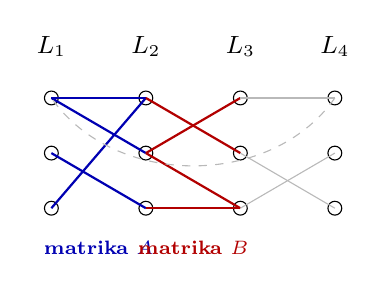
\begin{tikzpicture}[
          every node/.style={font=\scriptsize},
          vert/.style={circle,draw,inner sep=1.2pt,minimum size=5pt,fill=white},
          aedge/.style={blue!70!black,thick},
          bedge/.style={red!70!black,thick},
          cedge/.style={gray!55,thin},
        ]
        \foreach \xc/\lab in {0/$L_1$, 1.2/$L_2$, 2.4/$L_3$, 3.6/$L_4$} {
          \node[font=\small] at (\xc, 2.05) {\lab};
        }
        \foreach \xc in {0, 1.2, 2.4, 3.6} {
          \foreach \y in {0, 0.7, 1.4} {
            \node[vert] at (\xc, \y) {};
          }
        }
        \draw[aedge] (0, 1.4) -- (1.2, 0.7);
        \draw[aedge] (0, 1.4) -- (1.2, 1.4);
        \draw[aedge] (0, 0.7) -- (1.2, 0);
        \draw[aedge] (0, 0) -- (1.2, 1.4);
        \draw[bedge] (1.2, 1.4) -- (2.4, 0.7);
        \draw[bedge] (1.2, 0.7) -- (2.4, 1.4);
        \draw[bedge] (1.2, 0.7) -- (2.4, 0);
        \draw[bedge] (1.2, 0) -- (2.4, 0);
        \draw[cedge] (2.4, 1.4) -- (3.6, 1.4);
        \draw[cedge] (2.4, 0.7) -- (3.6, 0);
        \draw[cedge] (2.4, 0) -- (3.6, 0.7);
        \draw[cedge,dashed] (3.6, 1.4) to[bend left=55] (0, 1.4);
        \node[blue!70!black, font=\scriptsize\bfseries] at (0.6, -0.5) {matrika $A$};
        \node[red!70!black, font=\scriptsize\bfseries] at (1.8, -0.5) {matrika $B$};
      \end{tikzpicture}

      \vspace{0.5em}
      {\scriptsize $A \cdot B$ je tabela 2-koračnih poti s prejšnje prosojnice.}
    \end{column}
    \begin{column}{0.58\textwidth}
      Vsako vozlišče 4-cikla s prejšnje prosojnice ima eno od štirih \alert{vlog}: položaj $1$, $2$, $3$ ali $4$.

      \medskip
      Plast $L_i$ je množica vseh vozlišč, gledanih kot kandidati za vlogo $i$ -- konceptualno gre za štiri kopije iste množice vozlišč.

      \medskip
      \alert{$A$}: povezave med kandidati za vlogi $1$ in $2$. \\
      \alert{$B$}: povezave med kandidati za vlogi $2$ in $3$.

      \medskip
      Produkt $A \cdot B$ nam za vsak par $(1, 3)$ pove, koliko je vmesnih vozlišč v vlogi $2$ -- natanko \alert{zgornja polovica} 4-cikla s prejšnje prosojnice.

      \medskip
      \alert{Hitro} množenje matrik ta produkt izračuna strogo hitreje kot naivni pristop -- prav to je bližnjica, ki prebije mejo $m^{2/3}$.
    \end{column}
  \end{columns}
\end{frame}

% ---------------------------------------------------------------
\begin{frame}{En matrični korak, podprt z ogrodjem}
  Določili smo ključni matrični korak. Vendar ostaja temeljna napetost:

  \vspace{0.5em}
  \begin{block}{Množično proti tokovnemu}
    Hitro množenje matrik je \alert{množično}: pričakuje dve celotni matriki, ki ju pomnožimo naenkrat.

    \medskip
    Naš problem je \alert{tokovni}: povezave prihajajo posamično, ena za drugo.
  \end{block}

  \vspace{0.6em}
  \alert{Vse ostale komponente algoritma obstajajo zato, da premostijo to vrzel:}
  \begin{itemize}
    \item Razdelitev vozlišč po stopnji $\to$ nadzor nad velikostjo in obliko matrik.
    \item Vzdrževanje po kosih $\to$ porazdelitev množičnega stroška na veliko povezav.
    \item Faze $\to$ ohranjamo pripravljen produkt iz prejšnje faze, medtem ko v ozadju računamo naslednji produkt.
  \end{itemize}

  \vspace{0.4em}
  Vsa ta kompleksnost ima en sam namen: omogočiti, da množično množenje matrik deluje pri tokovnih posodobitvah.
\end{frame}

% ---------------------------------------------------------------
\begin{frame}{Hitro množenje matrik je bistveno, ne le postransko}
  Bi pospešitev lahko izvirala iz katerega koli drugega dela mehanizma? Pokazali smo, da ne more.

  \vspace{0.8em}
  Sistem omejitev algoritma smo analizirali pri \alert{domnevno optimalnem} eksponentu množenja matrik.

  \vspace{0.8em}
  Sklep je oster:

  \vspace{0.4em}
  \begin{block}{\centering Če odstranimo korak hitrega množenja matrik, celotna pospešitev izgine -- meja pade nazaj na prejšnji $m^{2/3}$.}
  \end{block}

  \vspace{0.8em}
  Hitro množenje matrik je torej \alert{nosilni} korak. Vse okoliško ogrodje obstaja zgolj zato, da je ta korak uporaben v tokovnem okolju.
\end{frame}

% =========================================================================
% Govorec 4 -- Eksperimenti in povzetek (3:30)
% =========================================================================

% ---------------------------------------------------------------
\begin{frame}{Implementacija in eksperimentalna postavitev}
  Teorija nam pove, da je matrični korak nujen. Empirično vprašanje pa je: \alert{pri katerih vhodih se zapleten okoliški mehanizem dejansko splača?}

  \vspace{0.6em}
  \textbf{Trije sestavni deli, vsi v Pythonu:}
  \begin{itemize}
    \item \alert{Algoritem.} Zvesta implementacija strukture novega algoritma -- štiri plasti, pragi stopenj, vzdrževanje posodobitev po kosih in osrednji korak množenja matrik.
    \item \alert{Izhodišče.} Naravni, preprostejši pristop -- štetje klinov na istem štiriplastnem grafu, brez mehanizma za usmerjanje po razredih.
    \item \alert{Testno orodje.} Generator grafov z nadzorovano strukturo: naključni grafi, grafi z enostransko visoko stopnjo, grafi z obojestransko visoko stopnjo in grafi z enakomerno nizko stopnjo.
  \end{itemize}

  \vspace{0.4em}
  Oba algoritma poganjamo na enakih grafih in enakih tokovih posodobitev. Zanima nas \alert{režim, v katerem novi algoritem zmaga}, ne pa njegov asimptotični eksponent.
\end{frame}

% ---------------------------------------------------------------
\begin{frame}{Kdaj algoritem zmaga: obojestransko visoke stopnje}
  \begin{columns}[T]
    \begin{column}{0.52\textwidth}
      \centering
      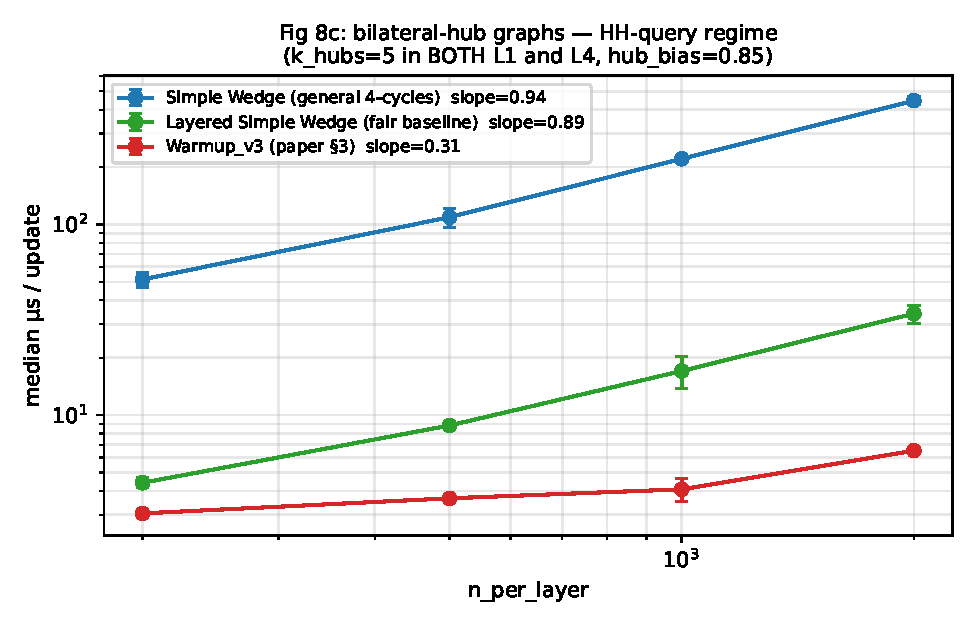
\includegraphics[width=\linewidth]{figures/fig8c_bilateral.pdf}
    \end{column}
    \begin{column}{0.48\textwidth}
      Novi algoritem prekaša izhodišče natanko takrat, ko ima graf \alert{vozlišča visoke stopnje na nasprotnih straneh} cikla:

      \vspace{0.4em}
      \centering
      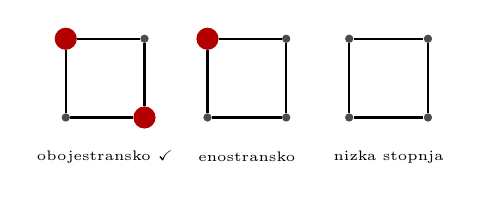
\begin{tikzpicture}[
          every node/.style={font=\tiny},
          hub/.style={circle,fill=red!70!black,inner sep=0pt,minimum size=8pt},
          small/.style={circle,fill=black!70,inner sep=0pt,minimum size=3pt},
        ]
        % Obojestransko
        \begin{scope}[xshift=-1.8cm]
          \node[hub]   (a) at (-0.5,0.5) {};
          \node[small] (b) at (0.5,0.5) {};
          \node[hub]   (c) at (0.5,-0.5) {};
          \node[small] (d) at (-0.5,-0.5) {};
          \draw[thick] (a)--(b)--(c)--(d)--(a);
          \node at (0,-1.0) {\alert{obojestransko} \checkmark};
        \end{scope}
        % Enostransko
        \begin{scope}[xshift=0cm]
          \node[hub]   (a) at (-0.5,0.5) {};
          \node[small] (b) at (0.5,0.5) {};
          \node[small] (c) at (0.5,-0.5) {};
          \node[small] (d) at (-0.5,-0.5) {};
          \draw[thick] (a)--(b)--(c)--(d)--(a);
          \node at (0,-1.0) {enostransko};
        \end{scope}
        % Brez vozlišč visoke stopnje
        \begin{scope}[xshift=1.8cm]
          \node[small] (a) at (-0.5,0.5) {};
          \node[small] (b) at (0.5,0.5) {};
          \node[small] (c) at (0.5,-0.5) {};
          \node[small] (d) at (-0.5,-0.5) {};
          \draw[thick] (a)--(b)--(c)--(d)--(a);
          \node at (0,-1.0) {nizka stopnja};
        \end{scope}
      \end{tikzpicture}

      \vspace{0.3em}
      V ostalih režimih izhodišče dosega skoraj enako učinkovitost; dodatni mehanizem postane le režija.

      \vspace{0.3em}
      Algoritem torej ni splošni pospeševalnik, temveč cilja na \alert{poseben strukturni režim}, v katerem se vzpostavitev hitrega množenja matrik dejansko izplača.
    \end{column}
  \end{columns}
\end{frame}

% ---------------------------------------------------------------
\begin{frame}{Povzetek}
  Iz dveh perspektiv pridemo do istega sklepa:
  \begin{itemize}
    \item \alert{Teoretično}: samo en korak je nosilen -- hitro množenje matrik.
    \item \alert{Empirično}: samo en režim resnično potrebuje celoten mehanizem -- obojestransko visoke stopnje.
  \end{itemize}

  \vspace{0.4em}
  Oba vidika kažeta, da okoliški mehanizem obstaja zgolj zato, \alert{da omogoči eno dobro pripravljeno množenje matrik}.

  \vspace{0.6em}
  \textbf{Smeri za nadaljnje delo:}
  \begin{itemize}
    \item Daljši cikli -- $k$-cikli za $k > 4$.
    \item Sprotno zaznavanje obojestranskega režima, sicer pa preklop nazaj na izhodiščni algoritem.
    \item Analiza v zaprti obliki pri \emph{trenutnih} eksponentih množenja matrik.
  \end{itemize}

  \vspace{0.3em}
  Širše gledano: gre za jasen vpogled v napetost med \alert{množičnim in tokovnim računanjem}, ki je prisotna povsod v dinamičnih podatkovnih sistemih.
\end{frame}

% ---------------------------------------------------------------
\begin{frame}[standout]
  Hvala. \\[0.5em]
  \large Vprašanja?
\end{frame}

\end{document}
